\chapter{Paths in Graphs}
\section{Connectivity}
Imagine you are developing a game, where the map is generated automatocally.
In this gate there are several areas connected by portals. So you need to check
that all the areas in your map are reachable from one another.

First we need to somehow understand what we mean by ``reachable'', we say that
an area $A$ is reachable from an area $B$ if there is a path from $A$ to
$B$. To formalize this notion using graphs we need to intrduce a graph
corresponding to the map, consider a graph $G = (V, E)$ such that vertices of
the graph are areas in your map and $(A, B) \in E$ iff the areas $A$ and $B$
are connected by a portal. So a path from $A$ to $B$ is a sequence of areas
$A = C_1$, \dots, $C_\ell = B$ such that $C_i$ and $C_{i + 1}$ are connected by
a portal (i.e. $(C_i, C_{i + 1}) \in E$).
\begin{definition}
  Let $G = (V, E)$ be a graph. We say that a path from $u$ to $v$ is
  a sequence $w_1, \dots, w_\ell \in V$\footnote{%
    Usually such an object is called a walk, and it is called a path if
    all the vertices $w_1$, \dots, $w_\ell$ are different. However,
    for our applications it does not matter and we will use the word ``path''.
  } such that
  \begin{itemize}
    \item $w_1 = u$, $w_\ell = v$, and
    \item $(w_i, w_{i + 1}) \in E$ for $i \in [\ell - 1]$.
  \end{itemize}

  We say that $u, v \in V$ are connected iff there is a path from $u$ to $v$.
  So the graph is connected iff any $u, v \in V$ are connected.
\end{definition}
So, using this notatation, we need to check whether the graph corresponding to
the map is connected.

There are numerous ways to do it, we consider a simple algorithm just to see how
it works.
\begin{algorithm}
  \begin{algorithmic}[1]
    \Function{Connected}{$n$, $E$}
      \State $S \gets \emptyset$
      \State $Q \gets \set{1}$

      \While{$Q \neq \emptyset$}
        \State Choose an element $v$ from $Q$
        \State $Q \gets S \setminus \set{v}$

        \State $S \gets S \cup \set{v}$

        \State $Q \gets Q \cup
          \set[{(v, u) \in E \text{ and } u \notin S}]{u \in [n]}$
      \EndWhile
      \label{line:connectivity-last}
      \State \Return{$S = [n]$}
    \EndFunction
  \end{algorithmic}
  \caption{An algorithm checking whether the graph on $[n]$ with the set of
  edges $E$ is connected.}
  \label{algorithm:connectivity}
\end{algorithm}

\begin{theorem}
  Algorithm~\ref{algorithm:connectivity} checks whether the graph $([n], E)$
  is connected.
\end{theorem}
\begin{proof}
  To prove this we prove that $S$ is equal to the maximal connected subset $U$
  of $[n]$ containing $1$ (we say that a set $U$ is connected iff $G[U]$ is
  connected).

  It is easy to see that $S \subseteq U$.
  Assume that $U \neq S$ on line~\ref{line:connectivity-last}.
  Let $u \in U \setminus S$. Consider a sequence $N_i$ such that
  $N_0 = \set{u}$ and $N_{i + 1} = \set[{u \in N_i, (u, v) \in E}]{v \in [n]}$.
  Note that if a vertex $w \notin S$ on line~\ref{line:connectivity-last}, then
  all the neighbours of $w$ are not $S$. It is also clear that $N_{n} = U$.
  Therefore $S = \emptyset$ which is a contradiction.
\end{proof}

\section{Eulerian Paths}

Graph theory originated from a simple question asked by Leonard Euler:
``Is it possible to walk through the town of K\"{o}nigsberg, starting and
ending at the same place, so that we use each bridge exactly once?'' (the map of K\"{o}nigsberg is depicted on Figure~\ref{figure:konigsberg}).
\begin{figure}
  \begin{center}
    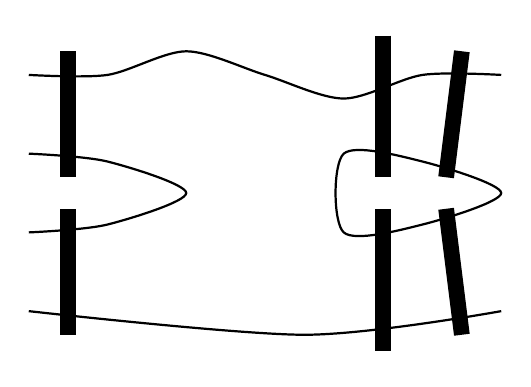
\begin{tikzpicture}[thick]
      \draw plot [smooth] coordinates {(0,0) (1, 0) (2,0.3) (3,0) (4,-0.3) (5, 0) (6, 0)};
      \draw plot [smooth] coordinates {(0, -3) (3.5, -3.3) (6, -3)};

      \draw plot [smooth] coordinates {(0,-1) (1, -1.1) (2, -1.5) (1, -1.9) (0,-2)};

      \draw plot [smooth cycle] coordinates {(4, -1) (5, -1.1) (6, -1.5) (5, -1.9) (4, -2)};

      \draw [line width=2mm] (0.5, 0.3) -- (0.5, -1.3);
      \draw [line width=2mm] (0.5, -3.3) -- (0.5, -1.7);
      \draw [line width=2mm] (4.5, 0.5) -- (4.5, -1.3);
      \draw [line width=2mm] (4.5, -3.5) -- (4.5, -1.7);
      \draw [line width=2mm] (5.5, 0.3) -- (5.3, -1.3);
      \draw [line width=2mm] (5.5, -3.3) -- (5.3, -1.7);
    \end{tikzpicture}
  \end{center}
  \caption{K\"{o}nigsberg's map}
  \label{figure:konigsberg}
\end{figure}
It is possible to see that the geometry of the islands is not inportant for
this problem, the only important property is the number of bridges between
islands.

In other words, all the necessary information can be described by the graph
(the islands are vertices and the bridges are edges) depicted on
Figure~\ref{figure:konigsberg-graph}.
\begin{figure}
  \begin{center}
    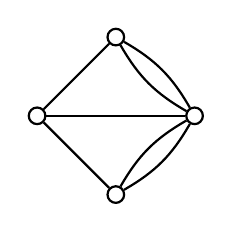
\begin{tikzpicture}[thick]
      \node[circle, draw, inner sep=0pt, minimum size=6pt] (v1) at (0,0) {};
      \node[circle, draw, inner sep=0pt, minimum size=6pt] (v2) at (1,1) {};
      \node[circle, draw, inner sep=0pt, minimum size=6pt] (v3) at (-1,1) {};
      \node[circle, draw, inner sep=0pt, minimum size=6pt] (v4) at (0,2) {};

      \draw (v4) to[out=-60, in=150] (v2);
      \draw (v4) to[out=-30, in=120] (v2);
      \draw (v1) to[out=60, in=-150] (v2);
      \draw (v1) to[out=30, in=-120] (v2);
      \draw (v2) -- (v3);
      \draw (v1) -- (v3);
      \draw (v4) -- (v3);
    \end{tikzpicture}
  \end{center}
  \caption{The graph of K\"{o}nigsberg's bridges}
  \label{figure:konigsberg-graph}
\end{figure}
Hence, to formalize the problem we need to give the following definition.
\begin{definition}
  A path $v_1$, \dots, $v_k$ in a graph $G = (V, E)$ is called Eulerian if for
  any edge $(u_1, u_2) \in E$ there is exactly one $i \in [k - 1]$ such that
  $u_1 = v_i$ and $u_2 = v_{i + 1}$.

  An Eulerian path is called an Eulerian cycle if $v_1 = v_k$.
\end{definition}
Using this definition the question is whether exists an Eulerian cycle in the
graph of K\"{o}nigsberg's bridges.

\begin{exercise}
  Check whether the graph of K\"{o}nigsberg's bridges has an Eulerian cycle or
  not.
\end{exercise}

The following theorem gives a simple criterion that allows us to solve the
problem in the general case.
\begin{theorem}
\label{theorem:eulerian}
  A connected graph $G$ has an Eulerian cycle if and only if all vertices
  of $G$ have even degree.
  (Note that the statement holds even if $G$ has parallel edges).
\end{theorem}

\begin{proof}
  Assume that such a cycle exists
  If a vertex $v$ appears $k$ times in the cycle, then there are $2k$ edges
  involving $v$ in the cycle (because, each time $v$ is visited, there is an
  edge used to step on $v$ and one to leave from $v$); since the cycle contains
  all the edges of the graph, $v$ has degree $2k$. Therefore all vertices have
  even degree. This shows that if a connected graph contains an Eulerian cycle,
  then every vertex has even degree.

  To prove ths statement in the other direction, we will prove by induction a
  stronger statement, we will prove that if $G$ is a graph in which every
  vertex has even degree, then every connected non-trivial connected
  component of $G$ (a connected component is trivial if it contains only an
  isolated vertex of degree zero) has an Eulerian cycle. We will proceed by
  induction on the number of edges.

  If there are zero edges, then every connected component has only one vertex
  and so it is nothing to prove. This is the base case of the induction.

  If we have a graph $G = (V,E)$ with a non-empty set of edges and in which
  every vertex has even degree, then let $V_1$, \dots, $V_m$ be the non-trivial
  connected components of $V$. If $m \ge 2$, then every connected component has
  strictly less vertices than $G$, and so we can apply the inductive hypothesis
  and find Eulerian cycles in each of $V_1$, \dots, $V_m$.

  It remains to consider the case in which the set $V'$ of vertices of non-zero
  degree of $G$ are all in the same connected component. Let $G' = G[V']$.
  Since every vertex of $G'$ has degree at least, there must be a cycle in
  $G'$. Let $C$ be a simple cycle (that is, a cycle with no vertices repeated)
  in $G'$, and let $G'' - C$. Since we have removed two edges from every
  vertex, we have that $G''$ is still a graph in which every vertex has even
  degree. Since $G''$ has fewer edges than $G'$ we can apply the induction
  hypothesis, and find an Eulerian cycle in each non-trivial connected
  component of $G''$. We can then patch together these Eulerian cycles with $C$
  as follows: we traverse $C$, starting from any vertex; the first time we
  reach one of the non-trivial connected components of $G''$, we stop
  traversing $C$, and we traverse the Eulerian cycle of the component, then
  continue on $C$, until we reach for the first time one of the non-trivial
  connected components of $G''$ that we haven’t traversed yet, and so on. This
  describes a Eulerian path into all of $G'$
\end{proof}

\begin{exercise}
  Finish the proof of Theorem~\ref{theorem:eulerian} by proving that if a graph
  $G$ has only vertices of an odd degree, then there is a simple cycle in $G$.
\end{exercise}

\begin{corollary}
  A graph $G$ has an Eulerian path starting and ending in two different
  vertices if and only if in $G$ there are exactly two vertices with odd
  degrees.
  (Note that the statement holds even if $G$ has parallel edges).
\end{corollary}
\begin{proof}
  Let $G = (V, E)$ and $u$ and $v$ be the vertices with odd degrees. Let us
  consider the graph $G + (u, v) = (V, E \cup (u, v))$ (if there are edges
  between $u$ and $v$ we increase their number by one). Note that all
  the degrees in $G + (u, v)$ are even.
  \nomenclature[G]{$G + e$}{denotes the graph $(V, E \cup \set{e})$}
  Therefore by Theorem~\ref{theorem:eulerian}, there is an Eulerian cycle in
  $G + (u, v)$. Without loss of generality the cycle is in the form $u$, $v$,
  $w_1$, \dots, $w_k$, $v$. Therefore, there is an Eulerian path $v$,
  $w_1$, \dots, $w_k$, $v$ in $G$.
\end{proof}

\section{Hamiltonian Paths}

Another example of a path that mathematicians are intrested is Hamiltonian path.
\begin{definition}
  Let $G$ be a graph. We say that a path in $G$ is Hamilton
  if it visits every vertex in $G$ exactly once. We say that such a path is a
  Hamiltonian cycle if its starting and ending vertices are
  connected.\footnote{%
    Hamiltonian paths and cycles are named after William Rowan Hamilton who
    invented the icosian game, now also known as Hamilton's puzzle, which
    involves finding a Hamiltonian cycle in the edge graph of the dodecahedron.
  }
\end{definition}

The greatest difference with Eulerian cycles is that it is not known whether
there is a fast (polynomial-time) algorithm that allows to find the Hamiltonian
cycles in a graph.\footnote{%
  Proving or disproving that there is a polynomial-time algorithm allowing to
  check whether a graph $G$ has a Hamiltonian path is one of the Millennium
  Problems. Clay Mathematics Institute offers a prise of \$1 million to a person
  who solves the problem.
}

It is easy to design an algorithm that checks whether a path exists in
$O((n - 1)!)$ by just brute forcing all the possible candidates for such a path.
However, using the ideas of the inclusion-exclustion principle, we may design
a much faster algorithm.
\begin{theorem}
  There is an algorithm such that it checks whether a graph $G$ on $n$ vertices
  has a Hamilton path in $O(2^n n^3)$ steps.
\end{theorem}

However, one may prove that if all the vertices in a graph have large degree,
then the graph has a Hamiltonian cycle.
\begin{theorem}[Dirac]
  Let $G$ be a graph on $n \ge 3$ vertices. If every vertex $v$ in $G$ has
  degree at least $n / 2$, then there is a Hamiltonian cycle in $G$.
\end{theorem}
